\documentclass[12pt,a4paper]{article}

%\usepackage[left=2cm, right=2cm, top=4cm, bottom=2cm]{geometry}
\usepackage[utf8]{inputenc}
\usepackage[spanish]{babel}
\usepackage{enumitem}
\usepackage{amsmath}
\usepackage{tikz}

\usepackage{hyperref}
\hypersetup{
    colorlinks=true,
    linkcolor=blue,
    filecolor=magenta,
    urlcolor=cyan,
}

\begin{document}

\begin{titlepage}
	\centering
	{\scshape\LARGE Universidad Nacional Autónoma de México \par}
	\vspace{1cm}
	{\scshape\Large Computación Distribuida\par}
	\vspace{1cm}
	{\huge\bfseries Algoritmos Autorregulables\par}
	\vspace{1cm}
    {\Large\itshape Jerónimo Almeida Rodríguez \par}
    \vspace{.5cm}
	{\Large\itshape Edgar Quiroz Castañeda \par}
    \vspace{.5cm}
	{\Large\itshape Naomi Reyes \dots \par}
	\vfill
	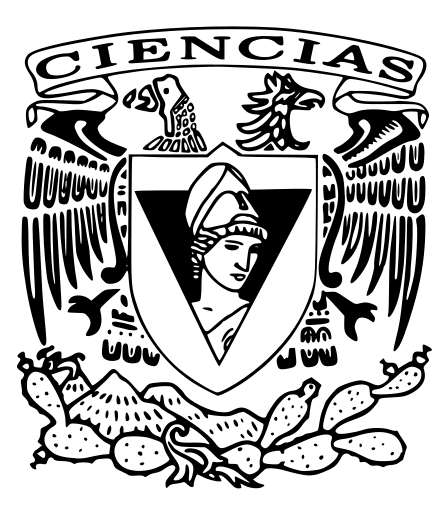
\includegraphics[width=0.5\textwidth]{escudo_f-ciencias.png}
	\vfill

	{\large Viernes 14 de Diciembre del 2018 \par}
\end{titlepage}

	\pagebreak
	\setlength{\voffset}{-0.75in}
	\setlength{\headsep}{5pt}


\begin{center}
		\textsc{\huge Algoritmos Autorregulables\\}
		\textit{Jerónimo Almeida, Edgar Quiroz, Naomi Reyes\\}
        14/12/2018
\end{center}




\section{Introducción}{
    Los algoritmos autorregulables son aquellos tienen la propiedad de que todos los procesos que ejecuten dicho algoritmo tiendan eventualmente a alcanzar un estado válido sin importar el estado actual en el que se encuentren, es decir, que pueden iniciar en cualquier estado arbitrario no válido o en caso de que haya ocurrido algún error que altere el estado, que el proceso llegue a un estado válido. Este estado válido se define en términos de los requerimientos del sistema.
\subsection{Motivación}{
    Con un algoritmo autorregulable buscamos que el sistema se recupere de un error sin intervención humana, es decir que dado un estado global arbitrario (particularmente uno que sea erróneo), dar un algoritmo que haga que el estado global eventualmente se vuelva válido.\\
    \indent En la década de los 70's, Edsger Dijkstra buscaba resolver el problema de exclusión mutua en anillos, así que publicó un artículo sobre transferencia de tokens en un sistema que podía iniciar con $n$ o con $0$ tokens pero se buscaba que eventualmente solo hubiera uno. Esto dio inicio al campo de la computación distribuida que actualmente se conoce cómo auto estabilización. Este campo además de abarcar miles de artículos, tiene su propia conferencia, el "\textit{International Symposium on Stabilization, Safety, and Security in Distributed Systems}".
}
\subsection{Especificación}{
    De los algoritmos autorregulables, sabemos que en general, un proceso no puede determinar "desde adentro" si el estado en el que está es válido o no, por lo que tener una bandera o indicador de la validez del estado no es la mejor opción, ya que algún agente malicioso podría cambiar esta bandera y hacer que el proceso crea que ha alcanzado un estado válido aunque esto no sea cierto. Esta es la razón por la que estos algoritmos no terminan, pues de hacerlo podrían terminar en un estado que no sea válido. En cambio, lo que hacen es que convergen hacia un estado válido, es decir que el proceso, por medio de esta subrutina, modifica su estado de tal manera que con cada ejecución se acerque mas a lo que es el estado válido. De esto, tenemos la garantía de que eventualmente el estado global del sistema va a ser válido. De igual manera, sabemos que una vez alcanzado un estado válido, mientras no hayan errores, este estado válido se mantendrá por el resto de la ejecución. Una ventaja de que el proceso no termine, es que si algun proceso comete un error, puede recuperarse de ese error y regresar a un estado válido.

}
\subsection{Modelo}{
    
}
}
\section{Pase de Token en un Anillo}{}
\section{Sincronizadores}{
    Después del error inicial, se puede considerar que no habrá más errores
    en el sistema. Entonces, el modelo es asícnrono sin fallas y se puede hacer
    todo lo mismo que en un modelo de este tipo, si bien se requieren algoritmos
    diferentes debido a las peculiaridades de comunicación del modelo.\\
    Una de las cosas que se puede hacer es un sincronizador.

    \subsection{Generalidades de sincronizadores}{
    Un sincronizador es algún programa que corre en paralelo al programa
    principal y permite determinar la ronda de comunicación en un momento dado
    en un sistema asíncrono. \\
    Con esto se puede asegurar que todos los procesos avancen sus rondas al
    mismo tiempo. Esto permite emular un sistema síncrono, pues si se sabe la
    ronda se puede garantizar que ningún proceso recibirá ningún mensaje de
    la ronda $r+1$ si algún otro proceso no ha enviado todas los mensajes de
    la ronda $r$.\\
    Hay dos tipos de sincronizadores. Puede ser globales, que sincronizan a
    toda la red. O pueden ser locales, que significan que sincronizan únicamente
    vecindades.\\
    Uno de los sincronizadores más simples es el sincronizador $\alpha$.
    }

    \subsection{Sincronizador $\alpha$}{
        La idea es que cada proceso avise a todos sus
        vecinos cuando pase a la siguiente ronda. Cuando un proceso recibe el
        aviso de ronda de todos sus entonces envía todos los mensajes de esa
        ronda, y pasa a la siguiente ronda.\\
        Puede pasar que un haya algún proceso $p_0$ ya haya enviado su aviso de
        ronda, pero que que aún no haya enviado todos los mensajes de la ronda
        $r$. Luego puede ser que algún $p_1 \in N(p_0)$ ya haya enviado todo y
        ya esté en la ronda $r+1$.\\
        $p_1$ no va a enviar ningún mensajes hasta que $p_0$ avise que ya avanzó de
        ronda, por lo que se respeta la regla de sinronización, pero las rondas
        de $p_0$ y $p_1$ difieren en 1.\\
        De esto, vemos que $\alpha$ es un sincronizador local.
        Y, en general, hay que notar que en cualquier momento cualesquiera dos nodos
        difieren a los más en una ronda.
    }

    \subsection{Sincronizador autorregulable}{
        La idea de un sincronizador autoregulable es que cada proceso comience
        con alguna ronda arbitraria, y que eventualmente se llegue y se
        permanezca en un estado válido para un sincronizador $\alpha$.\\
        Como en el modelo el estado de cada proceso es público para sus vecinos,
        no es necesario enviar mensajes al cambiar de ronda.\\
        Entonces, de las especificaciones del sincronizador $\alpha$, se tiene
        que lo único que un estado válido debe cumplir es que para todo par de
        procesos adyacentes, sus rondas difieran a lo más en 1.
    }

        \subsubsection{Regla Simple}{
        Intuitivamente, si los estados de los procesos son públicos para sus
        vecinos, lo más sencillo para ponerse de acuerdo en algún valor para la
        ronda sería tomar el mínimo.\\
        Pero esto generaría que los procesos se estanquen en ese mínimo, pues en
        cuanto algún otro proceso cmabie de ronda, inmediatamente volvería a ese
        mínimo.\\
        Y por la naturaleza del modelo, no es posible saber localmente cuando ya
        se llegó a un estado válido en el sistema.\\
        Entonces se puede siempre aumentar 1 a aquel mínimo en cada paso y
        esperar que eventualmente converga a un estado válido.\\
        La regla es entonces
        \[P(v) \leftarrow min_{w \in N(v)}(P(w)) + 1\]
        }

        \subsubsection{Segunda Regla}{}

        \subsubsection{Regla Óptima}{}
}
\section{Conclusión}{}

\begin{thebibliography}{}

\bibitem[Asp18]{Asp18}
James Aspnes. Notes on Theory of Distributed Systems.
\href{http://www.cs.yale.edu/homes/aspnes/classes/465/notes.pdf}
{http://www.cs.yale.edu/homes/aspnes/classes/465/notes.pdf}, October 2018.

\end{thebibliography}
\end{document}
